\documentclass[a4paper, runningheads, orivec]{llncs}

\usepackage{amsmath}
\usepackage{hyperref}
\usepackage{caption}
\usepackage{subcaption}
\usepackage{cleveref}
\usepackage[acronym]{glossaries}
\usepackage{tikz}
\usepackage{xcolor}

\setlength{\textfloatsep}{8pt plus 1pt minus 2pt}
\setlength{\floatsep}{6pt plus 1pt minus 2pt}
\setlength{\intextsep}{12pt plus 1pt minus 2pt}
\setlength{\abovecaptionskip}{4pt}
\setlength{\belowcaptionskip}{0pt}

\newacronym{spl}{SPL}{Standard Platform League}
\newacronym{hsl}{HSL}{Humanoid Soccer League}
\newacronym{ml}{ML}{Machine Learning}
\newacronym{cv}{CV}{Computer Vision}
\newacronym{cvat}{CVAT}{Computer Vision Annotation Tool}
\newacronym{sam}{SAM}{Segment Anything Model}
\glsdisablehyper

\definecolor{ballOrange}{RGB}{199, 92, 10}
\definecolor{fieldRed}{RGB}{245, 41, 5}
\definecolor{lineGreen}{RGB}{70, 199, 10}
\definecolor{robotCyan}{RGB}{10, 193, 199}
\definecolor{backgroundBlue}{RGB}{45, 10, 199}
\definecolor{goalPurple}{RGB}{199, 10, 193}

\begin{document}

\title{A Large Image Dataset for Robot Soccer in Diverse Competition Environments}

\titlerunning{A Large Image Dataset for Robot Soccer}

\author{Franziska-Sophie Göttsch\inst{1,2}\orcidID{0009{-}0001{-}9055{-}217X} \and Maximilian Schmidt\inst{1,2}\orcidID{0009{-}0005{-}4532{-}7669}}

\institute{Hamburg University of Technology, Hamburg, Germany \and
	HULKs e.V., RoboCup HSL Team Hamburg, Germany\\
	\email{hulks@tuhh.de}, \url{https://hulks.de}}

\maketitle

\begin{abstract}
	We present a large image dataset collected from Nao V6 humanoid robots in RoboCup soccer environments.
	It contains 1,864,394 images from multiple teams, venues, and years, manually categorized by environmental conditions such as lighting, shadows and reflections, line quality, and field color.
	A representative subset of 601 images is additionally annotated with pixel-wise segmentation masks for six semantic classes plus an uncertain label.
	By combining a large image corpus with semantic segmentation labels and manually assigned condition categories, the dataset enables targeted training and evaluation of robotic vision methods under realistic and challenging RoboCup conditions.

	Website: \url{https://hulks.de/nao-image-segmentation-dataset/}

	\keywords{Robot Soccer \and Image Dataset \and Semantic Segmentation \and Humanoid Robots \and RoboCup}
\end{abstract}

\glsresetall{}

\section{Introduction}

Data-driven methods require large amounts of diverse, high-quality, and domain-specific data with accurate annotations.
Collecting and annotating such datasets is time-consuming and costly.

In the RoboCup \gls{hsl} and former \gls{spl}, computer vision is essential for object detection, obstacle avoidance, and self-localization in autonomous soccer matches~\cite{qianAdaptiveFieldDetection2017}.
The RoboCup community's long-term goal of playing against human players by 2050 motivates increasingly realistic and challenging field conditions, including varying lighting, inconsistent artificial turf, shadows, reflections, and faded field markings.
These challenges highlight the need for datasets that provide not only images and labels, but also metadata describing the recording conditions.

To address this need, we present a large dataset of images captured by Nao V6 robots across multiple teams and events.
The contribution is twofold: first, the dataset provides nearly two million images from real RoboCup environments, including a manually segmented subset; second, each game is manually categorized by relevant environmental conditions, enabling targeted training and evaluation for conditions such as lighting, shadows, line quality, and field color.

\section{Dataset}

The dataset contains 1,864,394 images captured by Nao V6 robots across multiple teams and events.
It is archived in TORE, the TUHH research data repository, and released under the CC BY 4.0 license~\cite{goettsch2026dataset}.
Of these images, 601 are manually annotated with segmentation masks as described in~\Cref{subsec:annotations}.
Approximately 44\% of the images originate from our own team, \textit{HULKs}; the remainder comes from \textit{B-Human}, \textit{SPQR}, \textit{Nao Devils}, \textit{BerlinUnited}, and \textit{Dutch Nao Team}.
For each game, metadata records the image format and manually assigned environmental conditions.

\begin{figure}
	\centering
	\begin{tikzpicture}
		{
			\node[anchor=north west] at (0,0) {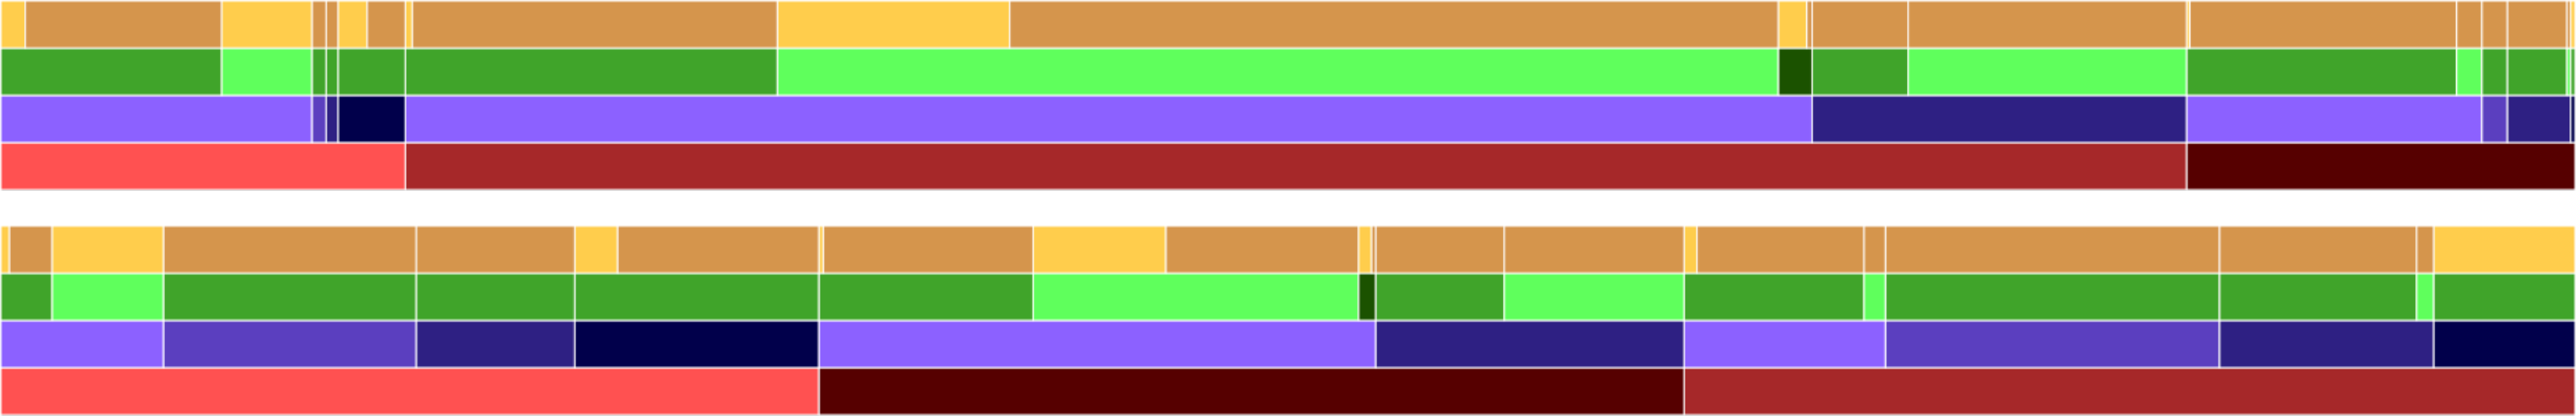
\includegraphics[width=0.95\textwidth, height=3.4cm]{figures/full_and_labeled_dataset_distribution.png}};

			\node[rotate=90, anchor=center] at (-0.1,-0.9) {\scriptsize \textbf{Full}};
			\node[rotate=90, anchor=center] at (-0.1,-2.75) {\scriptsize \textbf{Labeled}};
		}

	\end{tikzpicture}
	{
	\scriptsize
	\noindent
	\tikz[baseline=-0.6ex]\draw[fill={rgb,255:red,255; green,81; blue,81}, draw=none, yshift=-0.2em] (0,0) rectangle (4pt, 4pt); Sunlight\;
	\tikz[baseline=-0.6ex]\draw[fill={rgb,255:red,166; green,40; blue,41}, draw=none, yshift=-0.2em] (0,0) rectangle (4pt, 4pt); Artificial light\;
	\tikz[baseline=-0.6ex]\draw[fill={rgb,255:red,86; green,0; blue,0}, draw=none, yshift=-0.2em] (0,0) rectangle (4pt, 4pt); Mixed\;
	\tikz[baseline=-0.6ex]\draw[fill={rgb,255:red,140; green,97; blue,255}, draw=none, yshift=-0.2em] (0,0) rectangle (4pt, 4pt); None\;
	\tikz[baseline=-0.6ex]\draw[fill={rgb,255:red,91; green,63; blue,191}, draw=none, yshift=-0.2em] (0,0) rectangle (4pt, 4pt); Reflections\;
	\tikz[baseline=-0.6ex]\draw[fill={rgb,255:red,46; green,32; blue,131}, draw=none, yshift=-0.2em] (0,0) rectangle (4pt, 4pt); Shadows\;
	\tikz[baseline=-0.6ex]\draw[fill={rgb,255:red,1; green,0; blue,75}, draw=none, yshift=-0.2em] (0,0) rectangle (4pt, 4pt); Both\;
	\tikz[baseline=-0.6ex]\draw[fill={rgb,255:red,95; green,255; blue,92}, draw=none, yshift=-0.2em] (0,0) rectangle (4pt, 4pt); Taped\;

	\tikz[baseline=-0.6ex]\draw[fill={rgb,255:red,64; green,164; blue,42}, draw=none, yshift=-0.2em] (0,0) rectangle (4pt, 4pt); Spray-painted (fair)\;
	\tikz[baseline=-0.6ex]\draw[fill={rgb,255:red,27; green,82; blue,0}, draw=none, yshift=-0.2em] (0,0) rectangle (4pt, 4pt); Spray-painted (poor)\;
	\tikz[baseline=-0.6ex]\draw[fill={rgb,255:red,255; green,184; blue,0}, draw=none, yshift=-0.2em] (0,0) rectangle (4pt, 4pt); Inconsistent field color\;
	\tikz[baseline=-0.6ex]\draw[fill={rgb,255:red,196; green,104; blue,0}, draw=none, yshift=-0.2em] (0,0) rectangle (4pt, 4pt); Consistent field color
	}
	\caption{Distribution of images across light source (red shades), reflection/shadow (purple shades), line (green shades), and field (orange shades) conditions. The top plot corresponds to the full dataset, while the bottom plot shows the labeled subset.}\label{fig:dataDistribution}
\end{figure}

\subsection{Overview}

The dataset is organized hierarchically by game, robot, and camera.
Each top-level folder represents a single game and is identified by a unique game ID that references an entry in the metadata file.
This metadata file records the year, location, competing teams, and number of robots.
Within each of the 166 game folders, subfolders represent individual robots that participated in that game and contain two camera folders for the top and bottom camera images.

The dataset covers recordings from 2019 to 2025, including competitions such as RoboCup and GermanOpen, as well as team spaces and smaller event settings.
Images from the top camera are provided at a resolution of 640×480 pixels and make up roughly half of the dataset.
Images from the bottom camera are mostly 640×480 pixels, with a small subset at 320×240 pixels.
All images are stored in PNG or JPEG format and use RGB or YCrCb color spaces.

In addition to the technical metadata, each game is manually categorized by environmental factors affecting robot soccer vision.
These condition labels make it possible to select images for specific situations and to evaluate models on challenging subsets.
We distinguish the following categories:

\begin{itemize}
	\item \textbf{Light Source and Intensity}: Sun (medium), Sun (bright), Artificial (dark), Artificial (medium), Mixed (one side bright, one side dark)
	\item \textbf{Shadows and Light Reflections}: None, Reflections, Shadows, Both
	\item \textbf{Line Conditions}: Taped, Spray-painted (fair), Spray-painted (poor)
	\item \textbf{Field Conditions}: Inconsistent field color, Consistent field color
\end{itemize}

\Cref{fig:dataDistribution} compares the full dataset and labeled subset of 601 images across these four condition groups.
Because pixel-wise annotation is costly, the labeled subset is sampled to reflect the broader condition distribution, making it suitable for representative supervised experiments and condition-specific evaluations.
\Cref{fig:examplesDataset} shows several example images from the dataset.

\subsection{Image Segmentation Masks}\label{subsec:annotations}

The dataset includes segmentation masks for 601 manually labeled images (see \Cref{fig:examplesSegmentation}) covering six semantic classes: \textit{field}, \textit{lines}, \textit{ball}, \textit{robots}, \textit{goal}, and \textit{others} (e.g., background or humans), plus an \textit{uncertain} label.
Pixels assigned to the uncertain class include boundary regions between other classes, as well as areas that humans cannot clearly distinguish.
The images are annotated in \gls{cvat} with assistance from \gls{sam}.

\begin{figure}
	\centering

	\begin{subfigure}[b]{0.16\textwidth}
		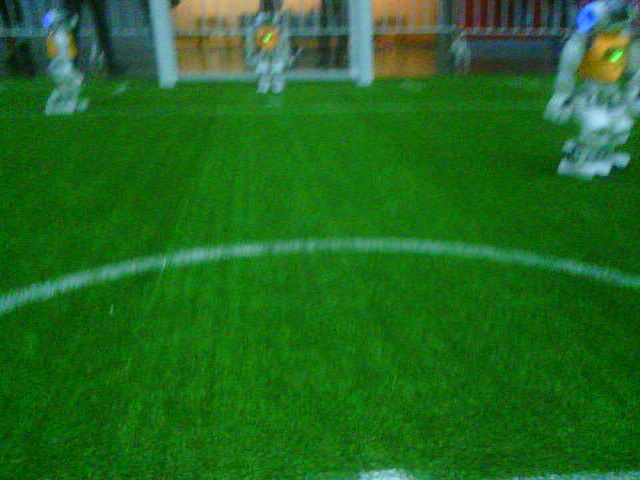
\includegraphics[height=1.45cm]{figures/00189_RGB.png}
	\end{subfigure}
	\begin{subfigure}[b]{0.16\textwidth}
		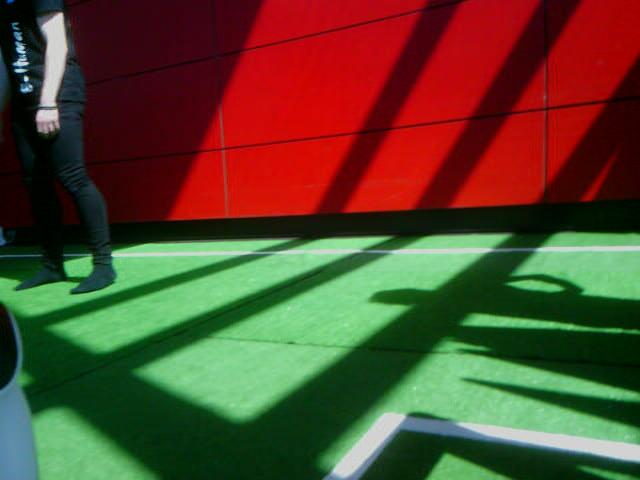
\includegraphics[height=1.45cm]{figures/00211_RGB.png}
	\end{subfigure}
	\begin{subfigure}[b]{0.16\textwidth}
		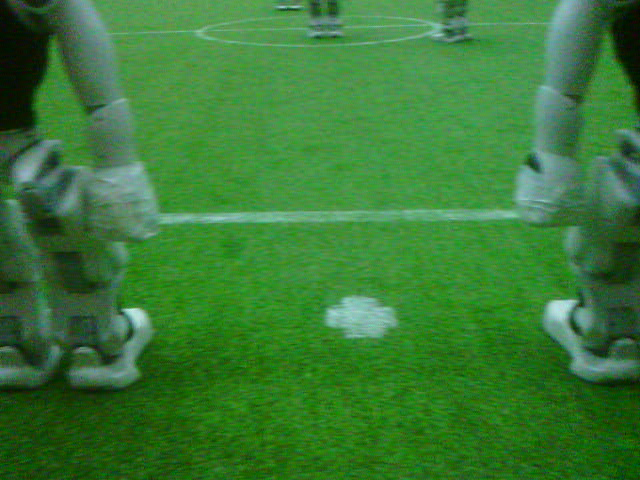
\includegraphics[height=1.45cm]{figures/00253_RGB.png}
	\end{subfigure}
	\begin{subfigure}[b]{0.16\textwidth}
		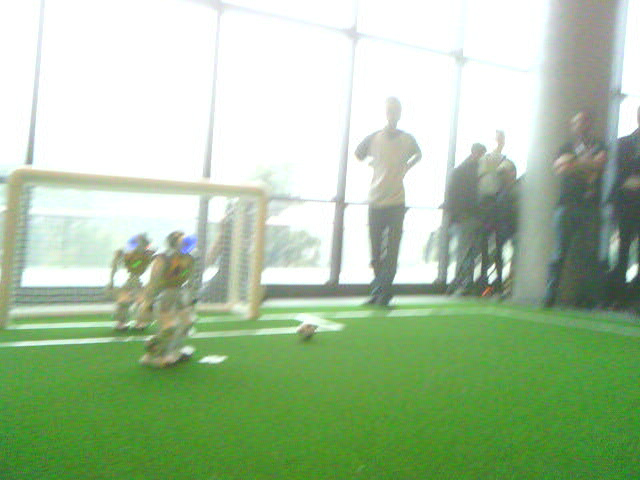
\includegraphics[height=1.45cm]{figures/00254_RGB.png}
	\end{subfigure}
	\begin{subfigure}[b]{0.16\textwidth}
		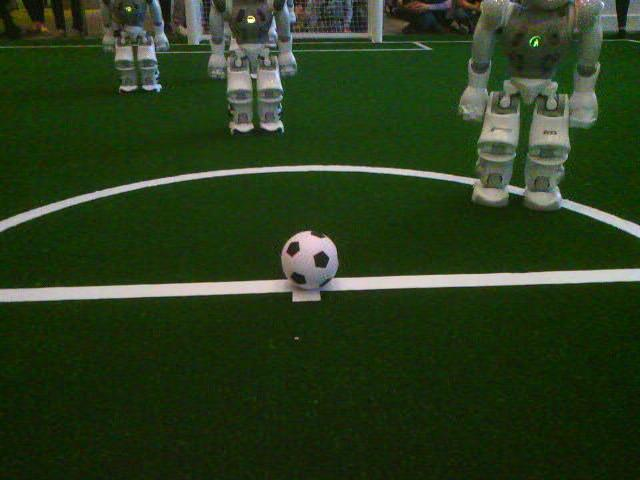
\includegraphics[height=1.45cm]{figures/00256_RGB.png}
	\end{subfigure}
	\begin{subfigure}[b]{0.16\textwidth}
		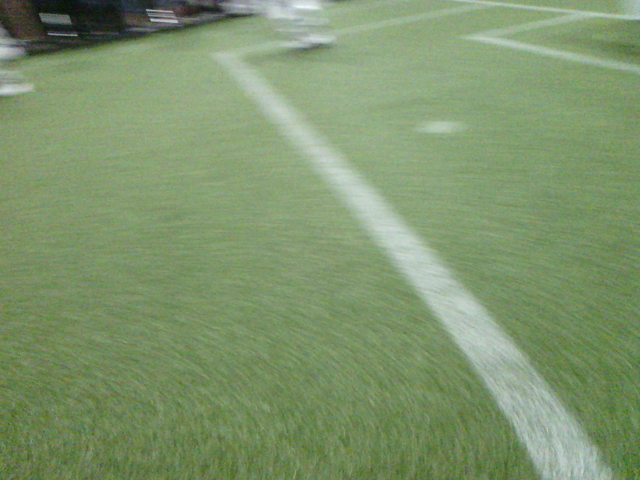
\includegraphics[height=1.45cm]{figures/00257_RGB.png}
	\end{subfigure}

	\vspace{0.3em}

	\begin{subfigure}[b]{0.16\textwidth}
		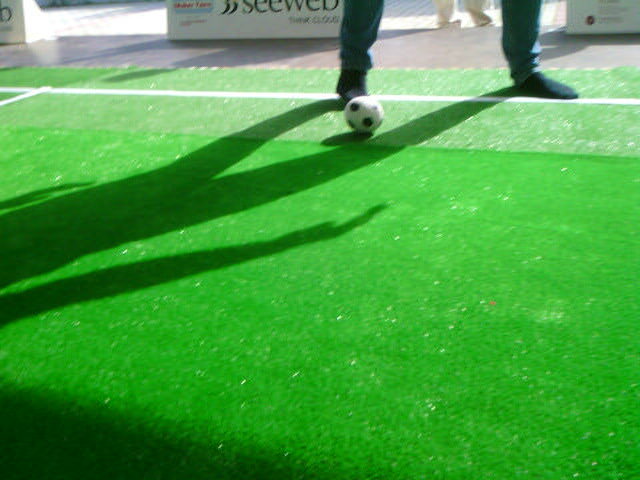
\includegraphics[height=1.45cm]{figures/00268_RGB.png}
	\end{subfigure}
	\begin{subfigure}[b]{0.16\textwidth}
		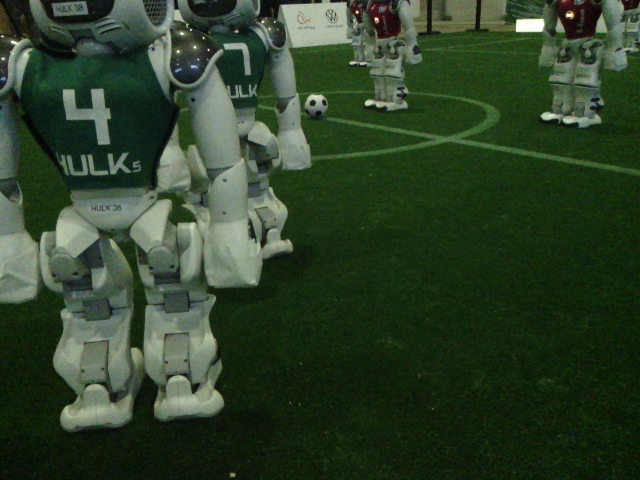
\includegraphics[height=1.45cm]{figures/00276_RGB.png}
	\end{subfigure}
	\begin{subfigure}[b]{0.16\textwidth}
		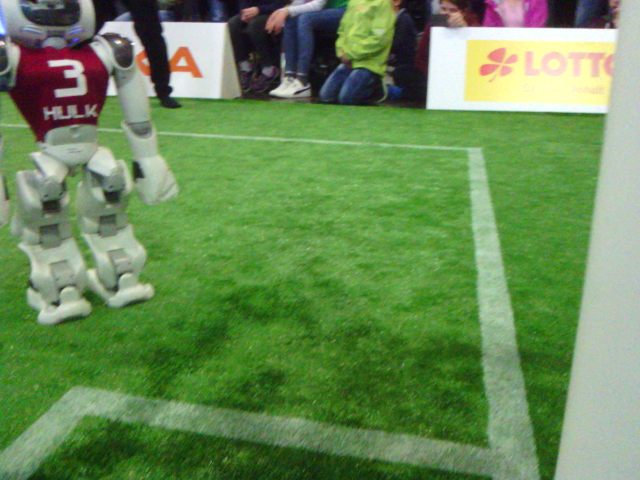
\includegraphics[height=1.45cm]{figures/00284_RGB.png}
	\end{subfigure}
	\begin{subfigure}[b]{0.16\textwidth}
		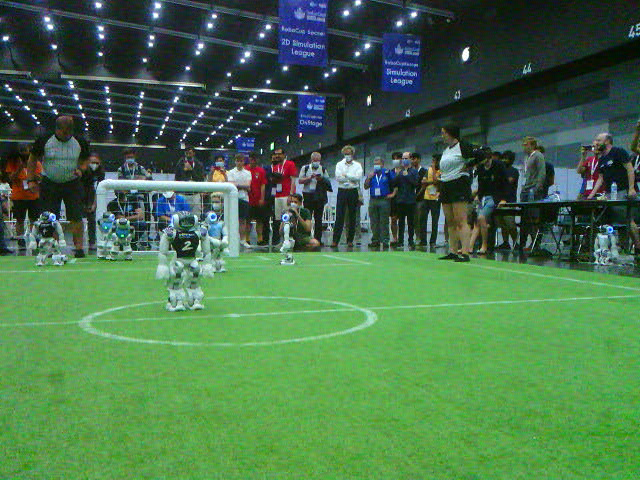
\includegraphics[height=1.45cm]{figures/00285_RGB.png}
	\end{subfigure}
	\begin{subfigure}[b]{0.16\textwidth}
		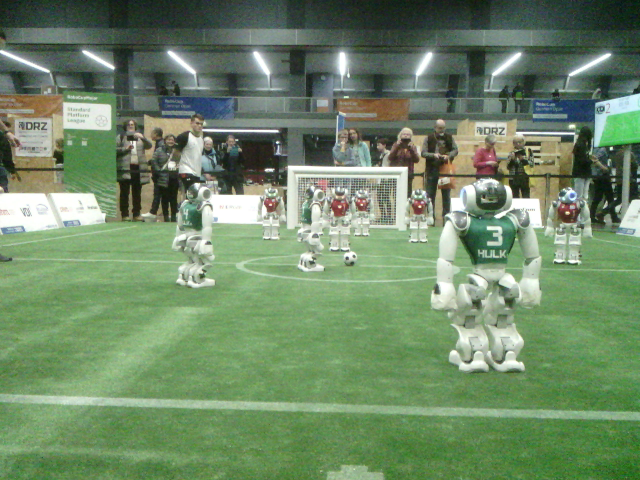
\includegraphics[height=1.45cm]{figures/00298_RGB.png}
	\end{subfigure}
	\begin{subfigure}[b]{0.16\textwidth}
		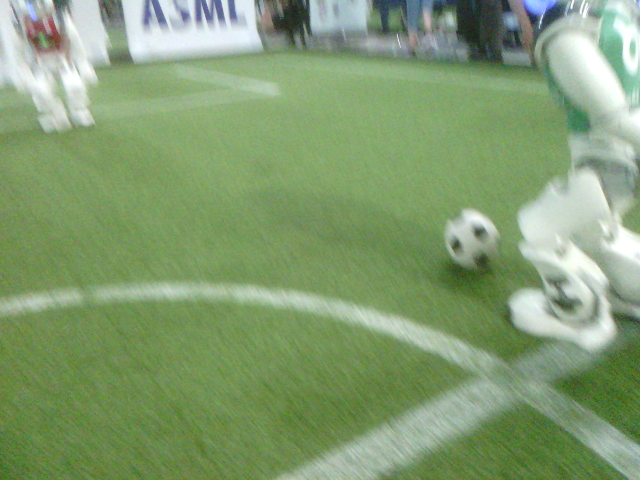
\includegraphics[height=1.45cm]{figures/00326_RGB.png}
	\end{subfigure}
	\caption{Example images of the dataset.}\label{fig:examplesDataset}
\end{figure}

\begin{figure}
	\centering
	\begin{subfigure}[b]{0.16\textwidth}
		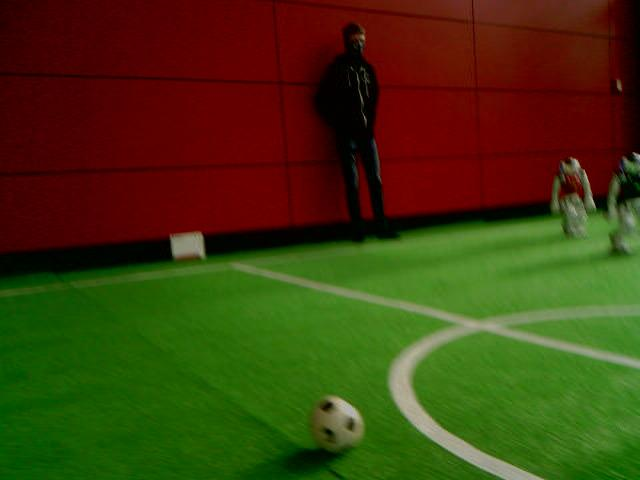
\includegraphics[height=1.45cm]{figures/00096_RGB.png}
	\end{subfigure}
	\begin{subfigure}[b]{0.16\textwidth}
		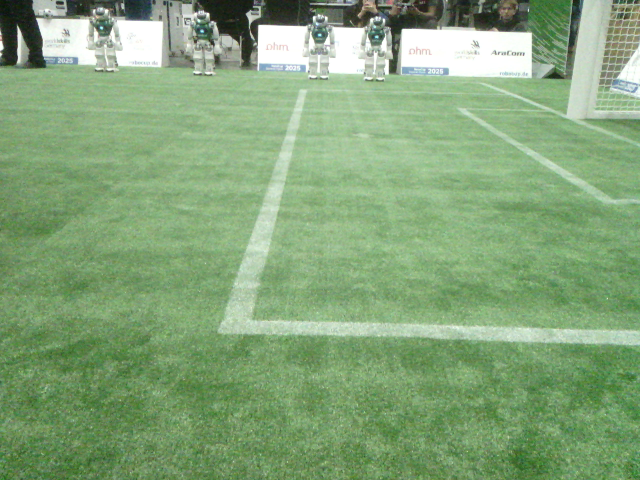
\includegraphics[height=1.45cm]{figures/00104_RGB.png}
	\end{subfigure}
	\begin{subfigure}[b]{0.16\textwidth}
		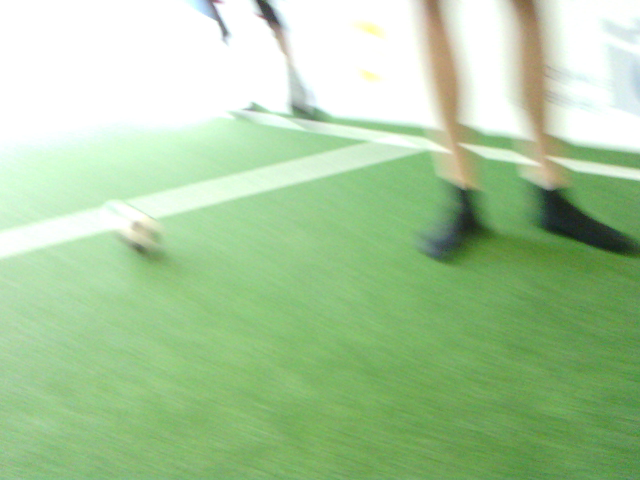
\includegraphics[height=1.45cm]{figures/00122_RGB.png}
	\end{subfigure}
	\begin{subfigure}[b]{0.16\textwidth}
		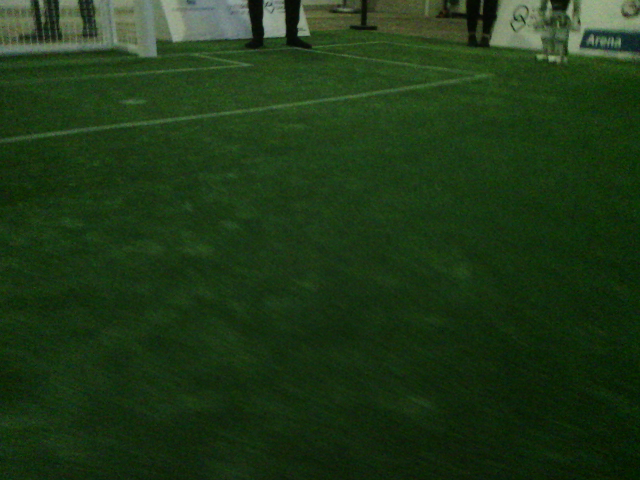
\includegraphics[height=1.45cm]{figures/00123_RGB.png}
	\end{subfigure}
	\begin{subfigure}[b]{0.16\textwidth}
		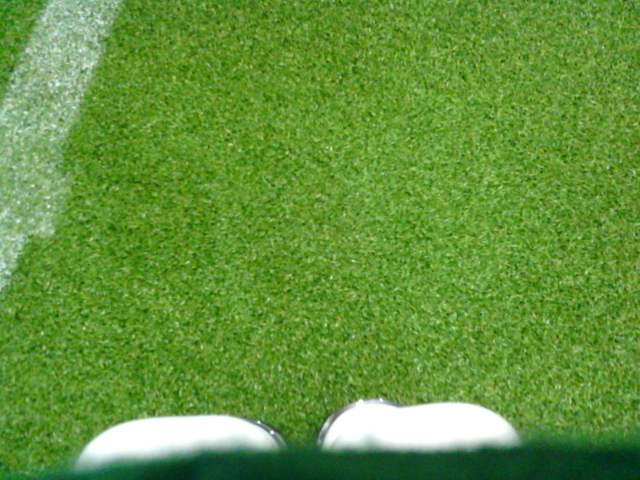
\includegraphics[height=1.45cm]{figures/00131_RGB.png}
	\end{subfigure}
	\begin{subfigure}[b]{0.16\textwidth}
		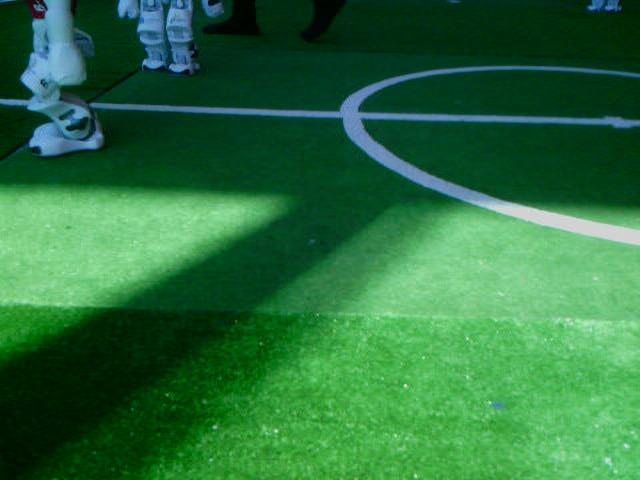
\includegraphics[height=1.45cm]{figures/00133_RGB.png}
	\end{subfigure}

	\vspace{0.3em}

	\begin{subfigure}[b]{0.16\textwidth}
		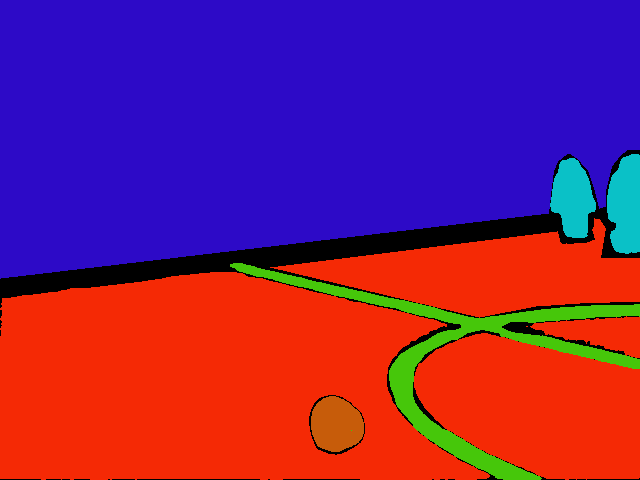
\includegraphics[height=1.45cm]{figures/00096.png}
	\end{subfigure}
	\begin{subfigure}[b]{0.16\textwidth}
		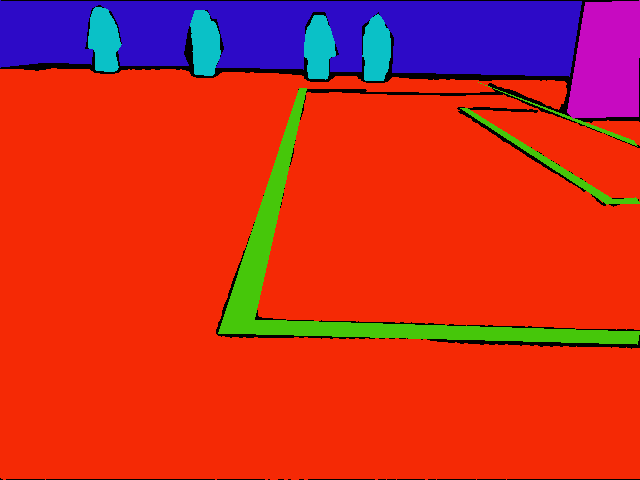
\includegraphics[height=1.45cm]{figures/00104.png}
	\end{subfigure}
	\begin{subfigure}[b]{0.16\textwidth}
		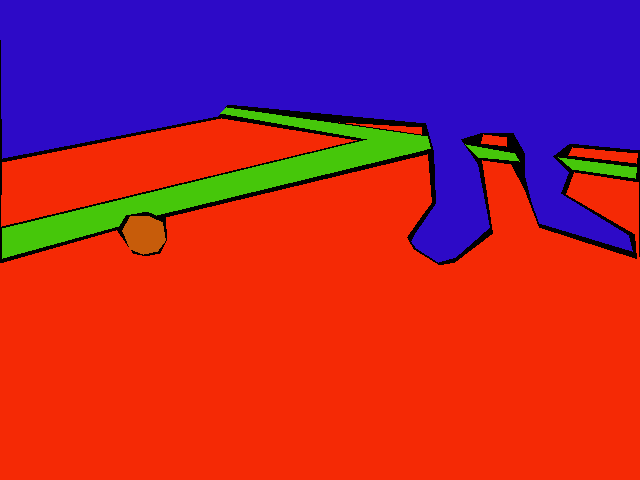
\includegraphics[height=1.45cm]{figures/00122.png}
	\end{subfigure}
	\begin{subfigure}[b]{0.16\textwidth}
		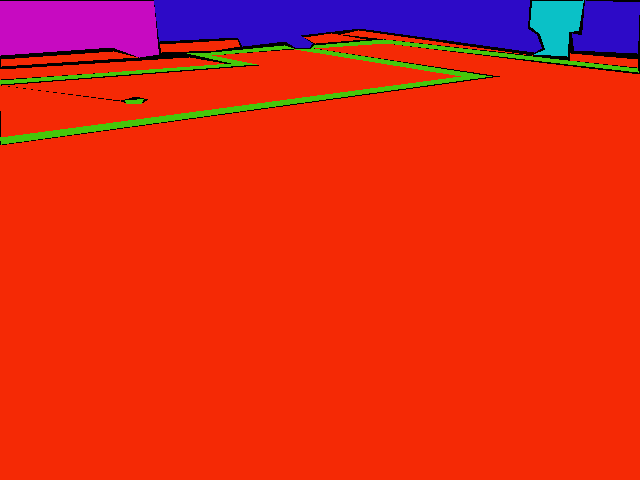
\includegraphics[height=1.45cm]{figures/00123.png}
	\end{subfigure}
	\begin{subfigure}[b]{0.16\textwidth}
		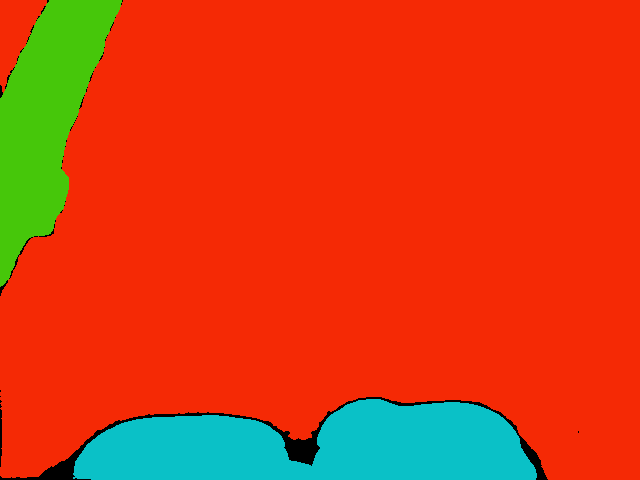
\includegraphics[height=1.45cm]{figures/00131.png}
	\end{subfigure}
	\begin{subfigure}[b]{0.16\textwidth}
		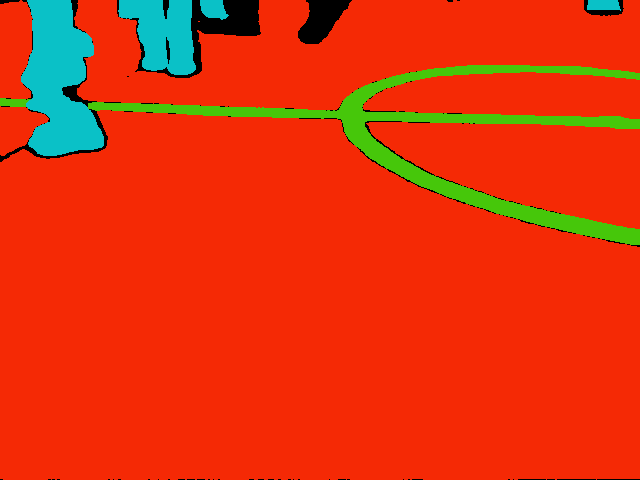
\includegraphics[height=1.45cm]{figures/00133.png}
	\end{subfigure}

	\vspace{0.3em}

	\begin{subfigure}[b]{0.16\textwidth}
		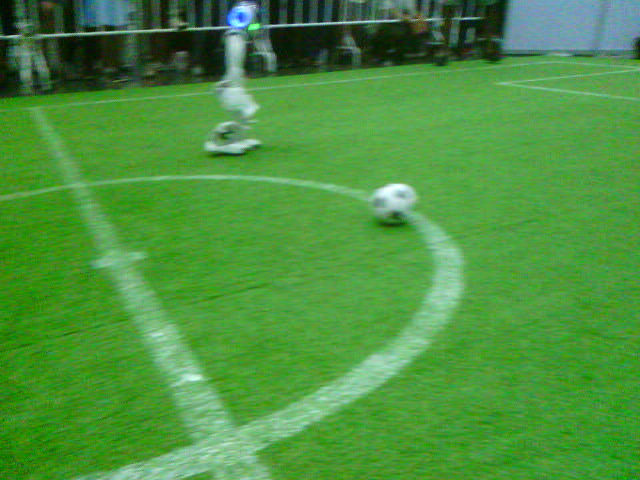
\includegraphics[height=1.45cm]{figures/00136_RGB.png}
	\end{subfigure}
	\begin{subfigure}[b]{0.16\textwidth}
		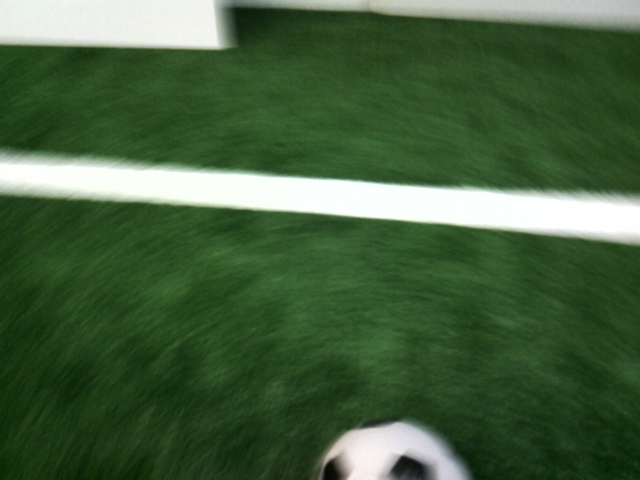
\includegraphics[height=1.45cm]{figures/00148_RGB.png}
	\end{subfigure}
	\begin{subfigure}[b]{0.16\textwidth}
		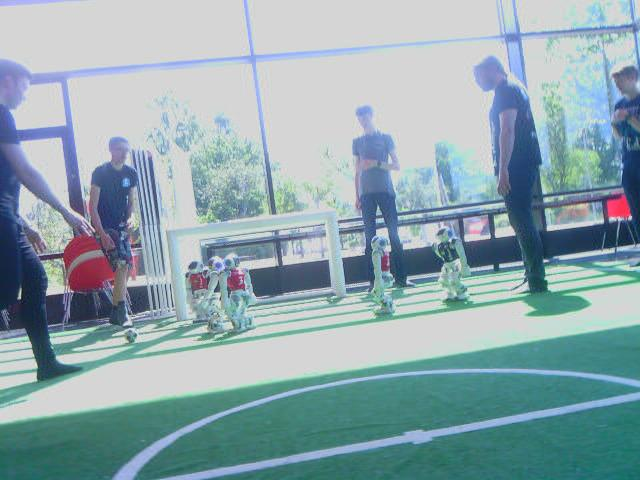
\includegraphics[height=1.45cm]{figures/00159_RGB.png}
	\end{subfigure}
	\begin{subfigure}[b]{0.16\textwidth}
		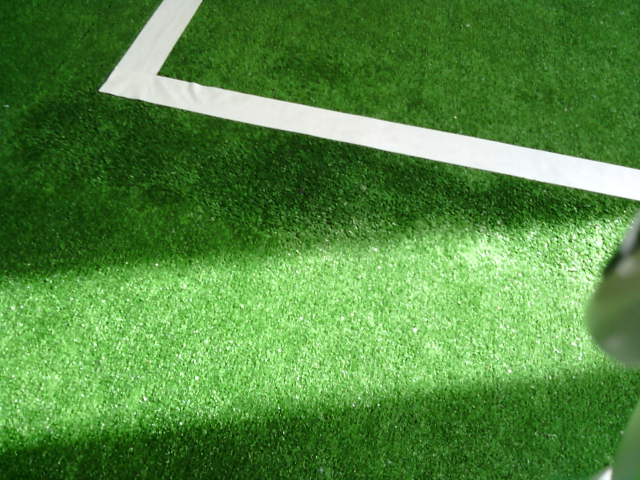
\includegraphics[height=1.45cm]{figures/00165_RGB.png}
	\end{subfigure}
	\begin{subfigure}[b]{0.16\textwidth}
		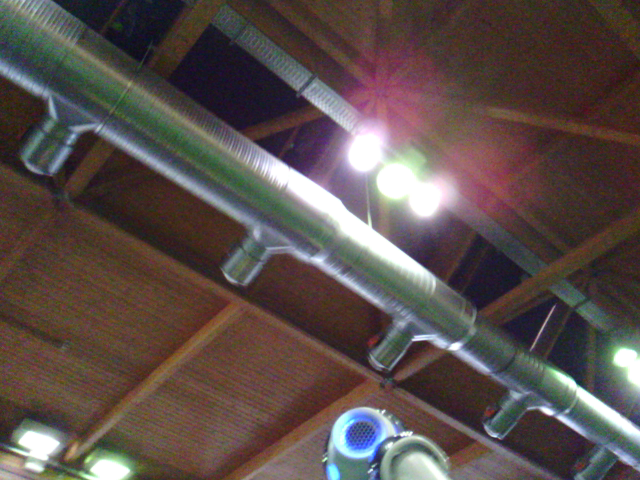
\includegraphics[height=1.45cm]{figures/00170_RGB.png}
	\end{subfigure}
	\begin{subfigure}[b]{0.16\textwidth}
		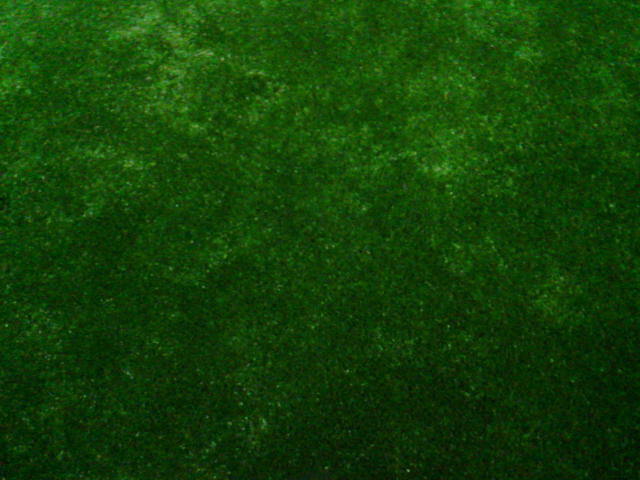
\includegraphics[height=1.45cm]{figures/00171_RGB.png}
	\end{subfigure}

	\vspace{0.3em}

	\begin{subfigure}[b]{0.16\textwidth}
		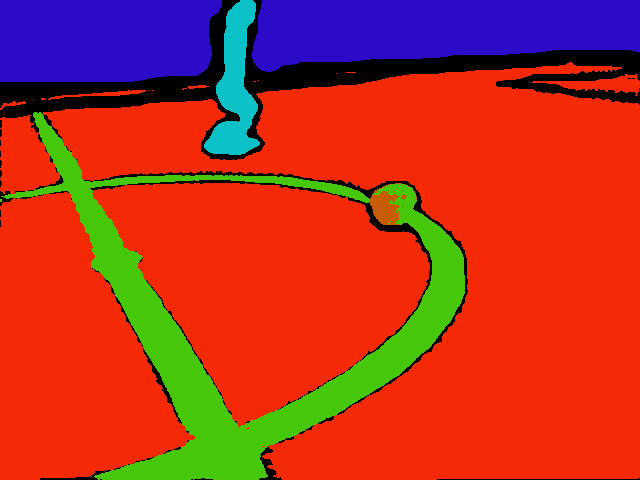
\includegraphics[height=1.45cm]{figures/00136.png}
	\end{subfigure}
	\begin{subfigure}[b]{0.16\textwidth}
		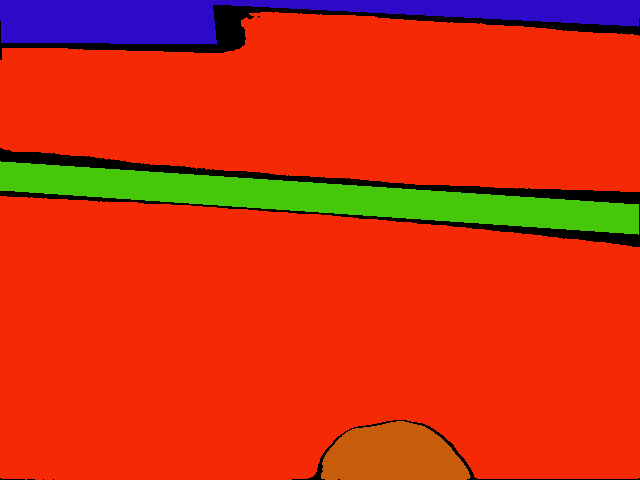
\includegraphics[height=1.45cm]{figures/00148.png}
	\end{subfigure}
	\begin{subfigure}[b]{0.16\textwidth}
		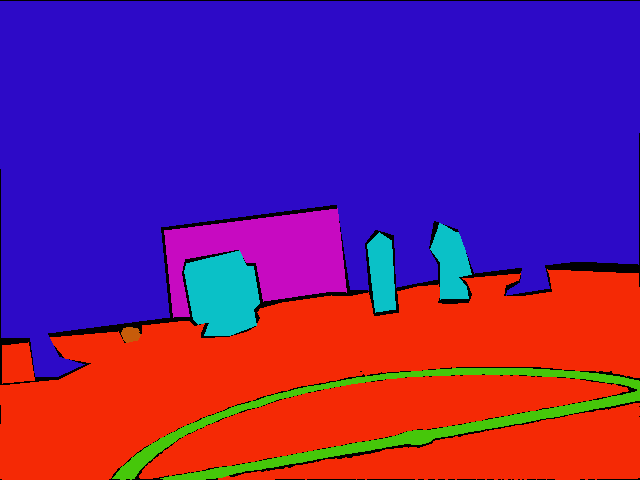
\includegraphics[height=1.45cm]{figures/00159.png}
	\end{subfigure}
	\begin{subfigure}[b]{0.16\textwidth}
		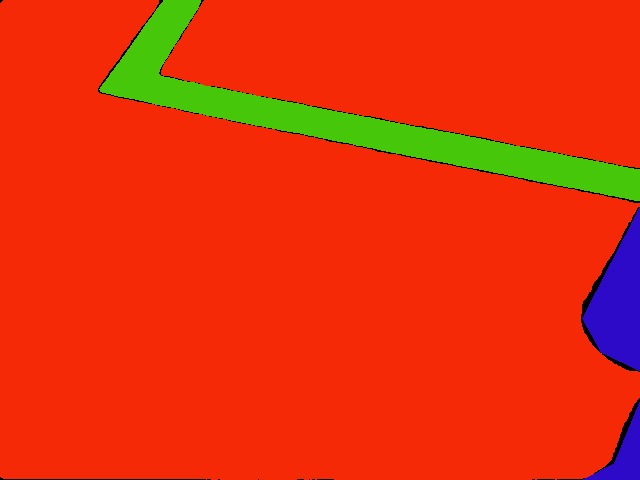
\includegraphics[height=1.45cm]{figures/00165.png}
	\end{subfigure}
	\begin{subfigure}[b]{0.16\textwidth}
		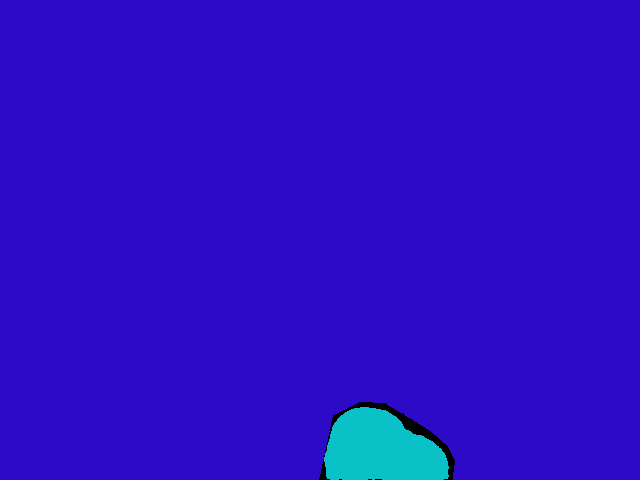
\includegraphics[height=1.45cm]{figures/00170.png}
	\end{subfigure}
	\begin{subfigure}[b]{0.16\textwidth}
		
\includegraphics[height=1.45cm]{figures/00171.png}
	\end{subfigure}

	\vspace{0.3em}

	\centering
	\begin{tabular*}{\textwidth}{@{\extracolsep{\fill}}lllllll}
		\tikz{\node[fill=fieldRed, minimum size=0.2cm] {};}\, Field &
		\tikz{\node[fill=lineGreen, minimum size=0.2cm] {};}\, Line &
		\tikz{\node[fill=ballOrange, minimum size=0.2cm] {};}\, Ball &
		\tikz{\node[fill=goalPurple, minimum size=0.2cm] {};}\, Goal &
		\tikz{\node[fill=robotCyan, minimum size=0.2cm] {};}\, Robot &
		\tikz{\node[fill=backgroundBlue, minimum size=0.2cm] {};}\, Others &
		\tikz{\node[fill=black, minimum size=0.2cm] {};}\, Uncertain
	\end{tabular*}
	\caption{Images from the labeled subset with corresponding segmentation masks.}\label{fig:examplesSegmentation}
\end{figure}

\section{Applications and Use Cases}

The dataset supports a range of applications in robotic vision.
The annotated subset can be used to train and evaluate segmentation models, while the large pool of unlabeled images supports custom annotation strategies and semi- or self-supervised learning~\cite{goettsch2026lightweight}.
With nearly 1.9 million images, the dataset provides sufficient scale for training robust models.
Although it is grounded in the RoboCup domain with Nao V6 robots, many aspects generalize to other robot soccer settings and related tasks.

A key advantage is the combination of environmental diversity and manual condition labels.
Because each game is categorized by lighting, shadows/reflections, line conditions, and field conditions, researchers can train models for specific scenarios, compare performance across environmental factors, and construct benchmark splits that isolate known failure cases.
These evaluations are difficult to perform from raw images and segmentation masks alone.

\section{Conclusion}

This dataset provides a comprehensive resource for training and evaluating robotic vision systems under realistic and diverse conditions. The large-scale unlabeled data, representative segmentation masks, and manual condition categories enable supervised and semi-supervised learning, targeted benchmarking, and domain adaptation research.
Future work includes expanding the dataset with additional annotations (e.g., bounding boxes or pose keypoints) and providing baseline results for common robotic vision tasks.

\section*{Acknowledgements}

We thank the teams \textit{B-Human}, \textit{SPQR}, \textit{Nao Devils}, \textit{BerlinUnited}, and \textit{Dutch Nao Team} for contributing to this dataset.

\bibliographystyle{splncs04}
\bibliography{literature}

\end{document}
